\review{The authors have addressed many of my previous comments. However, there are still several major issues that need further clarification.}

\vspace{0.1in}
We thank the reviewer for providing useful comments. The comments are constructive and helped us to improve the manuscript better.

\begin{enumerate}

\cmnt{1} \review{The revised paper did not address my previous comment about how to select the sub-channel ordering. I understand that finding the best sub-channel ordering requires exhaustive search which has extremely high complexity. But it is important to provide a guidance on what would be a good choice of sub-channel ordering. For example, can we achieve a good performance by using a low complexity ordering algorithm such as a greedy sub-channel ordering algorithm?}

\resp We apologize for not discussing the sub-channel ordering guidelines in a detailed manner. As suggested by the reviewer, we have included the guidelines on selecting the sub-channel ordering based on the greedy selection, which could be an educated guess over the random sub-channel ordering. Even though the number of backlogged packets must also be involved in the sub-channel ordering, greedy selection provides an effective ordering when the queues are fairly equal among the serving users or when the number of backlogged packets are significantly large. This information is now included in the revised manuscript under Section III-D final paragraph. We have included a plot comparing different ordering schemes to justify the above statement. Even though we are not including it in the paper, we have included in the response letter to justify the reviewers claim. We considered a system model with \eqn{N = 6} sub-channels, \eqn{N_B = 2} \acp{BS} with \eqn{N_T = 4} transmit antennas and \eqn{K = 12} single antenna users. The \ac{PL} is distributed uniformly over \eqn{[0,-3]} dB.
\begin{figure}[h!]
	\centering
	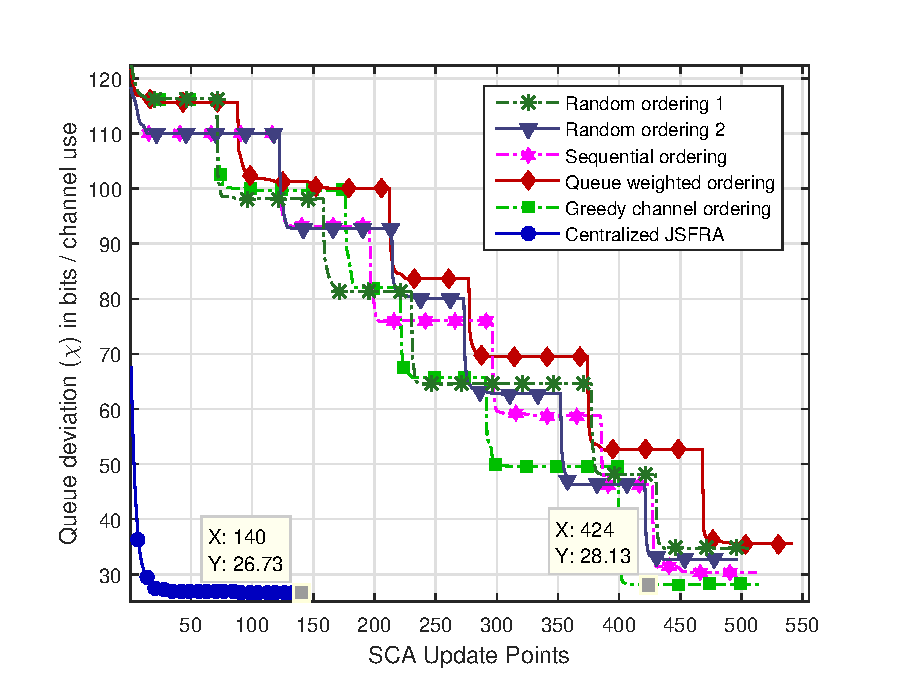
\includegraphics[width=0.8\columnwidth]{reviewer_2_Q1.eps}
	\caption{Convergence of the algorithms for \me{\lbrace N,N_B,K,N_T,N_R \rbrace = \lbrace 6,2,12,4,1 \rbrace} using \me{\ell_1} norm}
	\label{fig-review-1}
\end{figure}

Fig. \ref{fig-review-1} compares different ordering of sub-channels with the total number of backlogged packets remaining in the system as the metric. The random ordering are based on permutation of the sub-channel indices and sequential ordering is the natural way of selection. The greedy sub-channel ordering is based on sorting the best channel from each sub-channel, which is obtained by finding the highest channel norm between the users from the respective serving \ac{BS}. As pointed out by the reviewer, greedy scheduling performed much better when compared to the other random ordering schemes. 	

\cmnt{2} \review{The authors mentioned that the signaling overhead of the distributed algorithm can be reduced by using a smaller number of iterations \eqn{J_{\max}}. But still, you didn't answer my question about whether the signaling overhead of the distributed algorithm is smaller than the centralized algorithm. You should first analyze the signaling overhead of the distributed algorithm for fixed \eqn{J_{\max}} and the signaling overhead of the centralized algorithm. Then you should point out under what \eqn{J_{\max}} the distributed algorithm will have less signaling overhead than the centralized algorithm. Is it possible that the distributed algorithm always has more signaling overhead than the centralized algorithm even when \eqn{J_{\max} = 1}? Finally, there is a trade-off between performance and signaling overhead (\eqn{J_{\max}}) for the distributed algorithm. For the same signaling overhead (we can control \eqn{J_{\max}} to make the signaling overhead of the distributed algorithm approximately equal to that of the centralized algorithm), does the distributed algorithm achieve better performance than the centralized algorithm?}

\resp
	We thank the reviewer for the insightful comment and we apologize for the lack of clarity in explaining this information in our earlier manuscript.
	\begin{enumerate}
		\item Quantifying the signaling overhead of the distributed algorithm over the centralized one depends on the system model under consideration. For example, let us consider a model with \eqn{N = 1,N_B = 2,K = 4,N_T = 4,N_R = 1}, where each \ac{BS} has two users. In this scenario, the amount of information exchange to perform a centralized algorithm by a common controller requires the knowledge of complete channel matrices interlinked in the system, \textit{i.e}, the number of users times the \acp{BS}. In order to quantify the total number of bits required to be exchanged, let us assume that each complex channel for a single-input single-output requires \eqn{10} bits, \textit{i.e}, \eqn{4} bits for amplitude and \eqn{6} bits for phase (assuming phase is important). Using this assumption, the total number of channel information in bits to be exchanged via backhaul requires \eqn{10 \times K \times N_B \times N_R \times N_T \approx 320} bits. On the other hand, for the distributed case, let us consider \eqn{6} bits are required to quantize the scalar interference in the consensus vector. Therefore, it requires \eqn{6 \times 2 \times 2} bits of information to be exchanged for each iteration. With this overhead, we can perform only \eqn{6} \ac{SCA} updates with \eqn{J_{\max} = 2} internal iterations in each to reach the centralized overhead. Note that the number iteration includes the \ac{SCA} update as well. However, by knowing the complete channel of the users in the system, the centralized controller can perform the precoder design until convergence. However, as the number of sub-channels, users or the antenna element increases, it may not be a viable option to feedback the user channels across the coordinating \acp{BS} to the centralized controller. The quantizing the channel information degrades the achievable performance of the centralized solution that also needs to be considered while comparing the signaling overhead.
		\item Using the above discussion, we can say that when the system size is huge, it would be favorable to consider the distributed algorithm over the centralized approach due to the huge signaling overhead involved in exchanging the channels.
		\item In particular, \ac{ADMM} and primal approach requires significant overhead compared to the centralized algorithm when \eqn{J_{\max} = 1} for a small system, since by exchanging the quantized channels, each \ac{BS} can perform the centralized algorithm independently until convergence. However, it depends on the channel quantizer, which is likely to be based on the channel density function (eg. Lloyd quantizer). For a system involving more number of coordinating \acp{BS}, users and number of antenna elements, it would be beneficial to use distributed algorithm with \eqn{J_{\max} > 1} to have a strictly monotonic decrease in the objective.
		\item Even with the same signaling overhead, it is not possible to prove the benefits of the distributed algorithm like \ac{ADMM} and primal approach over the independent centralized scheme performed by exchanging the channel state information across the \acp{BS}. It is dependent on the system model under consideration. As explained earlier, for the considered system model, the independent centralized algorithm performs better in terms of the over head involved. 
	\end{enumerate}
	
	We have included the above information briefly in Section IV-C first paragraph and in the last paragraph. We have also included this information in the paragraph before the Conclusions section. Having said that, note that in reality, the channel is time-correlated, and it is often enough to update the precoders once per radio frame or certain number of symbols later. It is not necessary for the decentralized algorithm to converge until the end, it is only important to follow the fading process when \eqn{J_{\max} > 1}. The performance of the distributed algorithm based on dual decomposition scheme is discussed for the time-correlated fading in Section C of [13], which shows that it is enough for the distributed precoder design to follow the fading process to provide desired performance. The distributed algorithm for the time correlated case is not provided in the current manuscript, since it is not in the scope of the precoder design algorithms considered in this manuscript. However, for the clarity purpose, we have provided a plot demonstrating this behavior for the \ac{KKT} based algorithm in Section IV-C presented in the manuscript.
	\begin{figure}[h!]
		\centering
		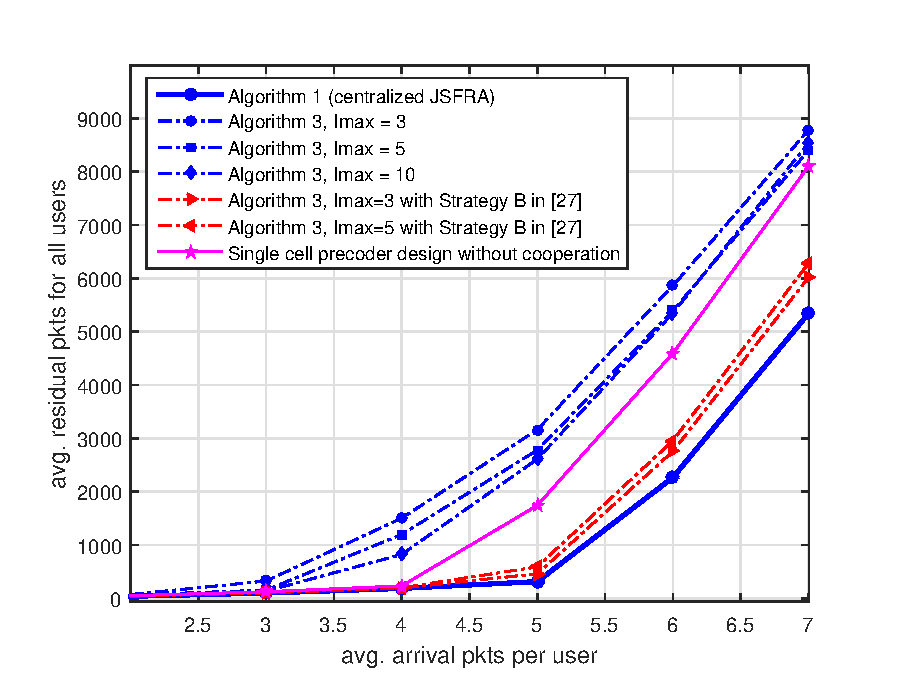
\includegraphics[width=0.8\columnwidth]{reviewer_2_Q2.eps}
		\caption{Average number backlogged packets after each transmission for system \me{\lbrace N,N_B,K,N_T,N_R \rbrace = \lbrace 4,2,16,4,2 \rbrace} evaluated for \eqn{500} slots}
		\label{fig-review-2}
	\end{figure}
		
	Fig. \ref{fig-review-2} compares the performance of the distributed \ac{KKT} approach presented in Section IV-C for different iteration. The signaling requirements are outlined in Algorithm 3 and the overhead involved in the signaling is penalized in the achievable rate of the users. We considered that the channel is coherent over \eqn{N_S = 100} symbols or frames and the precoder update is performed by exchanging the equivalent channel for \eqn{J_{\max} = 3,5,10} number of iterations. The overhead is considered as \eqn{\tilde{t}_{l,k,n} = (1 - \frac{J_{\max}}{N_S}) \times t_{l,k,n}}, where \eqn{\tilde{t}_{l,k,n}} is the rate seen by the user and the factor \eqn{(1 - \frac{J_{\max}}{N_S})} is considered as a penalty involved due to the precoder exchange. The average number of backlogged packets after each transmission slot is evaluated as 
	\begin{equation}
	\chi = \sum_{k = 1}^K \; [ Q_k - \tilde{t}_k ]^+
	\end{equation}
	Unlike the distributed algorithm, the centralized scheme presented in Fig. \ref{fig-review-2} has no penalty term and it is used as a benchmark for the other figures. In order to improve the performance of the distributed scheme, the operating point involved in the \ac{SCA} algorithm is considered from the earlier frame instead of starting initializing randomly. Since we use \ac{KKT} approach, we can either use all users in the system for the precoder design or we can utilize single-cell MU-MIMO user selection presented in the literature to limit the number of users for which the precoders are designed, which leads to the faster convergence. As we can see from Fig. \ref{fig-review-2}, as the arrival rate per user increases, the performance of \ac{KKT} schemes with \eqn{J_{\max} = 3,5,10} converges since the number of backlogged packets are significantly large, therefore, the same set of users will be served by the algorithm with better precoders by utilizing the memory. 
	
	In spite of using memory and prior scheduling in the \ac{KKT} approach, isolated single \ac{BS} processing performs much better than the distributed scheme due to the limited number of iterations allowed in the algorithm. Note that the precoders are not updated for the desired users until convergence, after the limited number of iterations. However, if we perform the single cell precoder design by considering the neighboring precoders as fixed after the recent exchange as discussed in [28], we can improve the performance significantly for Algorithm 3 as shown by red curves in Fig. \ref{fig-review-2}. In this approach, in between each exchange across the coordinating \acp{BS}, each \ac{BS} will perform \eqn{J_{\max} = 20} with the neighboring precoders as fixed. Once the iterations are performed to update the precoders, it is then exchanged across the coordinating \acp{BS} to perform the same procedure as mentioned earlier. 

\cmnt{3} \review{If the authors can't prove the convergence of the ADMM algorithm (or the decomposition approach via KKT conditions) in Section IV.B, then at least, you should discuss the property of the fixed point of the algorithm. For example, does there exist a fixed point of the algorithm? If so, is the fixed point of the algorithm unique? Is any fixed point of the algorithm also the optimal solution of the original problem in (20)? Assuming that the ADMM algorithm converges to a fixed point, will the interference vector in (39) converges to the actual interference in the network? These questions must be clarified in the paper. Otherwise, it is not clear how the ADMM algorithm is related to the original problem in (20). Similar questions should also be answered for the decomposition approach via KKT conditions. }

\resp We thank the reviewer for raising the important concern regarding the convergence issue of the distributed algorithm with limited number of iterations. In view of this, we have updated the manuscript to include the discussion on the convergence of the distributed algorithms with limited number of iterations in Appendix B third paragraph after (55). Since the distributed algorithm cannot be guaranteed to be monotonic in each iteration, it is not possible to prove the convergence of the algorithm. However, if the algorithm is allowed to converge or iterated to guarantee the monotonicity of the objective, it is possible to prove the convergence based on the discussions provided in the manuscript. 
\begin{itemize}
\item The fixed points for each convex subproblem exist, but may not be unique unless the objective function is regularized with a strongly convex term as discussed in Appendix A-C.
\item If the distributed algorithm is iterated for limited number of iterations, it is not guaranteed to achieve the fixed point even if the outer \ac{SCA} update is performed for large number of iterations. In this scenario, it is not guaranteed to converge. In all our simulations on the primal and the \ac{ADMM} approach, we have iterated \eqn{J_{\max} = 20} in order to guarantee the monotonicity of the objective.
\item Unless the objective function is regularized with a strongly convex term as in Appendix A-C, the uniqueness of the iterates is not guaranteed. 
\item In each \ac{SCA} update, if the distributed algorithm converges to a fixed point, then the overall convergence will be a stationary point of the original nonconvex problem. It may not be an optimal solution to the original nonconvex problem. It can be proved based on the strict monotonicity of the objective, since the distributed algorithm converges to a centralized solution.
\item Since the coupling between the distributed precoder designs are the interference between the BSs and the users, in the \ac{ADMM} approach, the interference is treated as a local variable, which is then included in the precoder design problem for each coordinating BS. This is treated as a local variable for a specific BS. Note that the local variable is an assumption made by the BS on the actual interference caused by the neighboring BSs. Since the actual interference caused is different, the consensus has to be made between the local interference variable maintained at each BS with the global consensus interference variable, which is nothing but the average between the corresponding BSs interference. These discussions have been made in the revised manuscript in Section IV-B. For further details we have also referred the interested reader to [11], which discusses exclusively about the ADMM approach. Upon convergence of the \ac{ADMM} approach, the interference vector can be considered as an upper bound of the actual interference seen in the network. It can be equal to the actual interference but not less.
\end{itemize}

\end{enumerate}
